\section{MTT Simulation Studies}
\label{sec:MTTsimulation}
	For future physics studies with MTT impact, this system has to be implemented in the standard CMS geometry description within CMSSW.
	In this section this implementation is described. 
	\subsection{MTT Geometry in CMSSW}
		\subsubsection{The geometry model of CMS}
			The geometry model of CMS is based on Geant4 \cite{Geant4}.
			It is constructed hierarchically and realized by the XML based detector description language \cite{CMSDDL}.
			To make the geometry available on runtime the ESProducer \verb+XMLIdealGeometryESSource+ is used converting the XML description of the geommetry in a C++ model.
			The tree structure of the geometry is then available in the event as an instance of the \verb+DDCompactView+.
			In general there are two main classes of geometries in CMS.
			For the tracking systems like the muon subdetectors and tracker etc. tracking geometries are available.
			For the calorimeter systems one can use the calorimetry geometry classes.
			Details on this procedure can be found in \cite{CMSDDL}.
			For alternative geometry models like the extended CMS geometry containing the MTT system it is nessessary to modify \verb+XMLIdealGeometryESSource+ to load corresponding XML
			files.
			In the next section the XML based geometry description of the MTT system is explained.
		\subsubsection{Description of the MTT geometry for different scenarios}
			\subsubsection*{General:}
			All parts of the MTT geometry are arranged in a hierarchy, which is very similar to the muon system hierarchy, especially of the DT system.
			Concerning this the MTT geometry is to be assigned to the class of tracking geometries.
			Furthermore the local coordinate system of MTT is chosen in a way, that the z axis concurs with the global z axis of CMS.
			The local y axis is therefore pointing outwards radially.
			\subsubsection*{Inner Hierarchy:}
			The basic unit of the MTT geometry is the \verb+MTTTile+.
			This unit is consisting of a scintillator of 10\,mm thickness wrapped by a polyethylene layer of 1\,mm thickness.
			In Figure \ref{fig:tile_wowrapping} several scintillators are seen in light green.
			The sensitive material of the scintillator is a generic hydrogencarbon compound with the mass composition of $m_H:m_C \approx 91.5\,\%:8.5\,\%$.
			\begin{figure}[htbp]
				\centering
				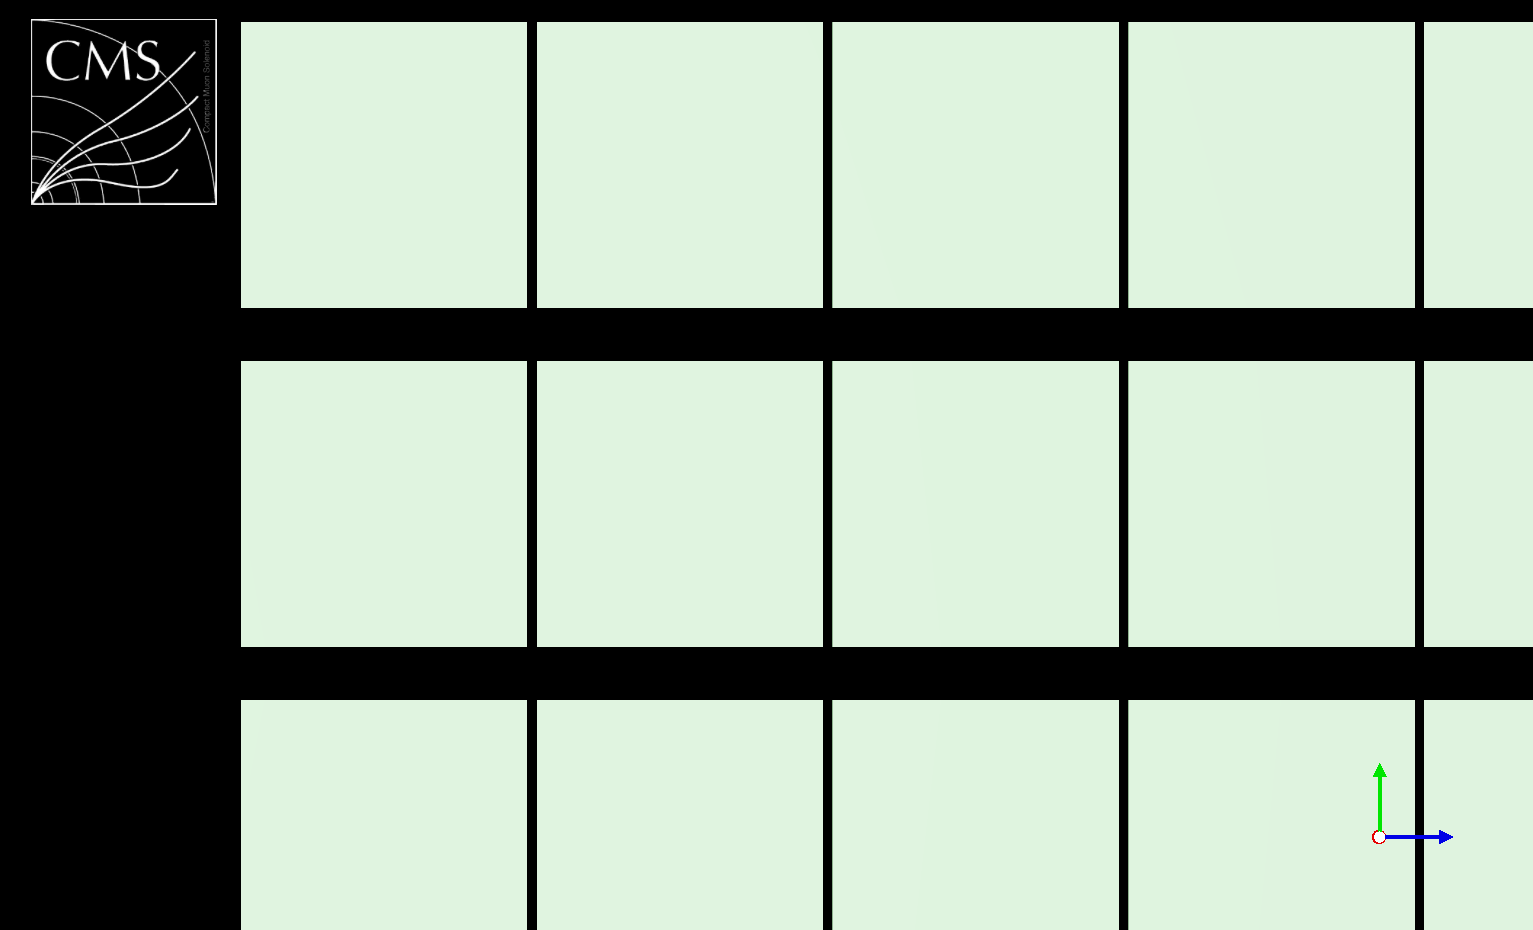
\includegraphics[width=0.70\textwidth]{Figures/erdogan/tile_wowrapping.png}
				\caption{MTT geometry: tiles without wrappings.}
				\label{fig:tile_wowrapping}
			\end{figure}
			The gaps in between are on the one side due to the absence of the wrapping and on the other side due to the placing in the superior detector unit called \verb+MTTStrip+.
			Several \verb+MTTTiles+ namely can be arranged along the z axis in these strips (Fig. \ref{fig:strip}).
			\begin{figure}[htbp]
				\centering
				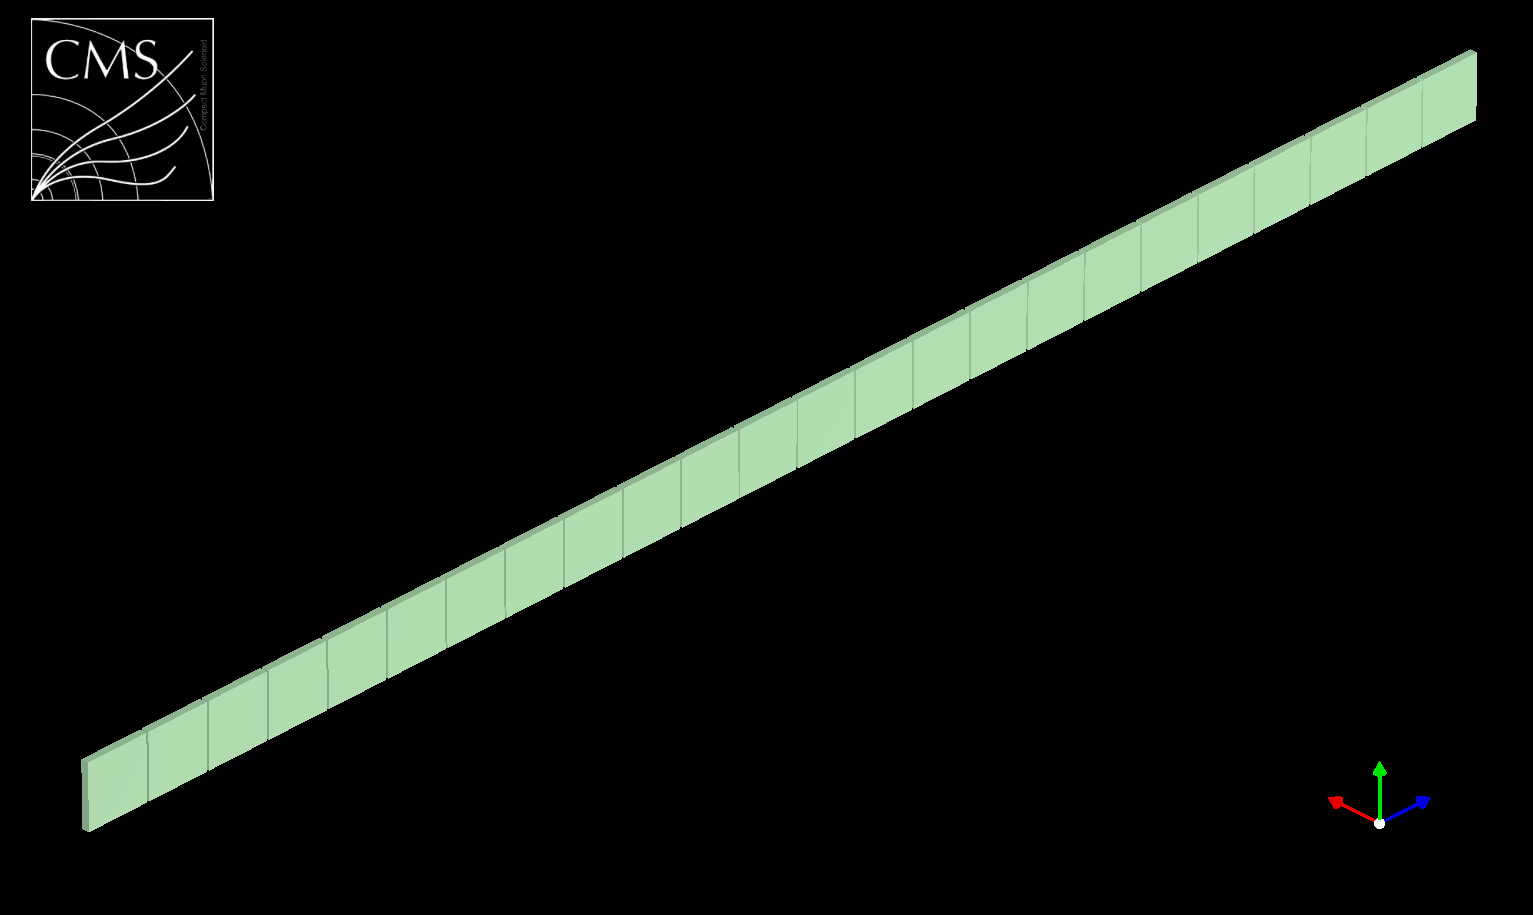
\includegraphics[width=0.70\textwidth]{Figures/erdogan/strip.png}
				\caption{MTT geometry: array of several tiles, called strip.}
				\label{fig:strip}
			\end{figure}
			The dimensions of the tiles are dynamic and determined automatically to be fit in a \verb+MTTStrip+ in a way that a strip contains the number of tiles given by the user having the insensitive areas
			between the tiles to be minimal.
			The dimension of a strip is fixed in z direction at 2536\,mm since this is the width of the wheels.
			This constraint is the reason of the insensitive areas between the tiles.
			However in a more sophisticated geometry description these areas can be minimalized since the implemented geometry is a first try to check the feasibility. 
			The strip itself is made of polystrene.
			An array of strips in local x direction is called a layer (Fig. \ref{fig:layer}).
			\begin{figure}[htbp]
				\centering
				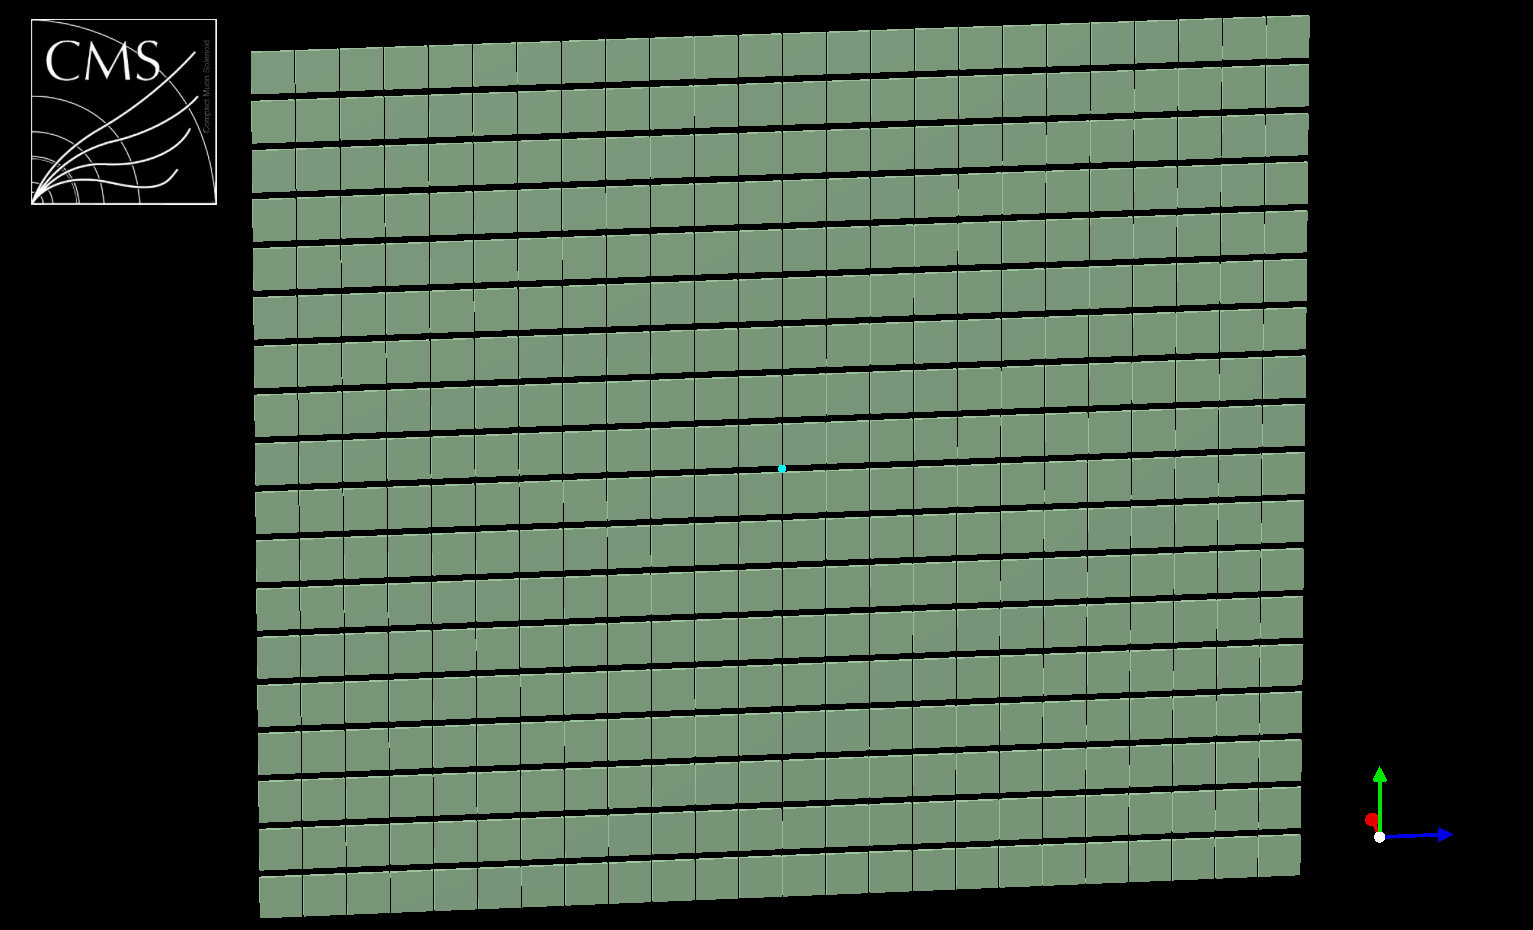
\includegraphics[width=0.70\textwidth]{Figures/erdogan/layer.png}
				\caption{MTT geometry: array of several strips, called layer.}
				\label{fig:layer}
			\end{figure}
			Several layers in y direction can be arranged in a panel, which is the top unit in the hierarchy.
			There are already different scenarios written for MTT geometry having one or more layers in a panel (Fig. \ref{fig:panel}).
			\begin{figure}[htbp]
				\centering
				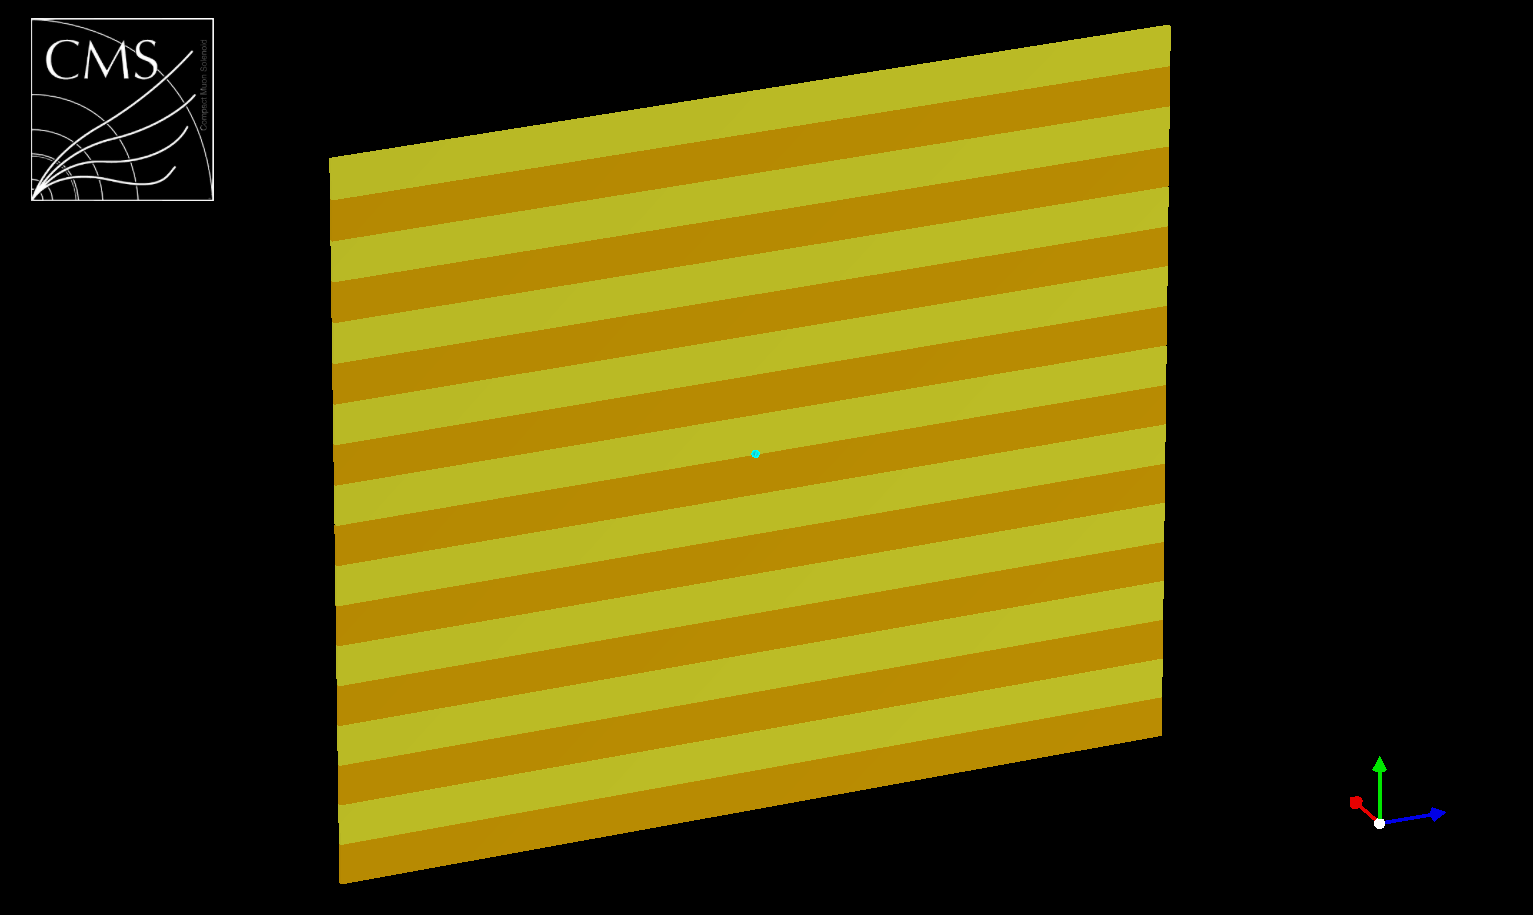
\includegraphics[width=0.45\textwidth]{Figures/erdogan/panel1.png}
				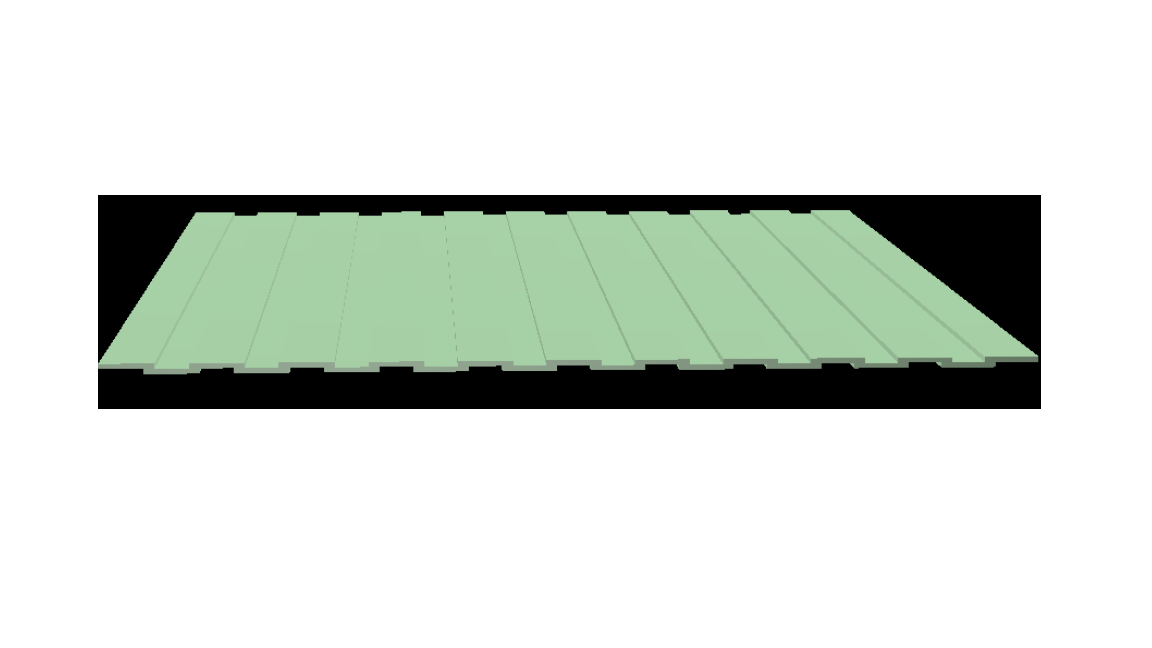
\includegraphics[width=0.45\textwidth]{Figures/erdogan/panel2.png}
				\caption{left: one MTTPanel with one layer, right a possible scenario for one panel with two layers.}
				\label{fig:panel}
			\end{figure}
			\subsubsection*{Numbering:}
			In the detector description of CMS, each detector unit is unique by a 32 bit integer named the DetId.
			The composition of this integer is depicted in Fig. \ref{fig:numbering}.
			\begin{figure}[htbp]
				\centering
				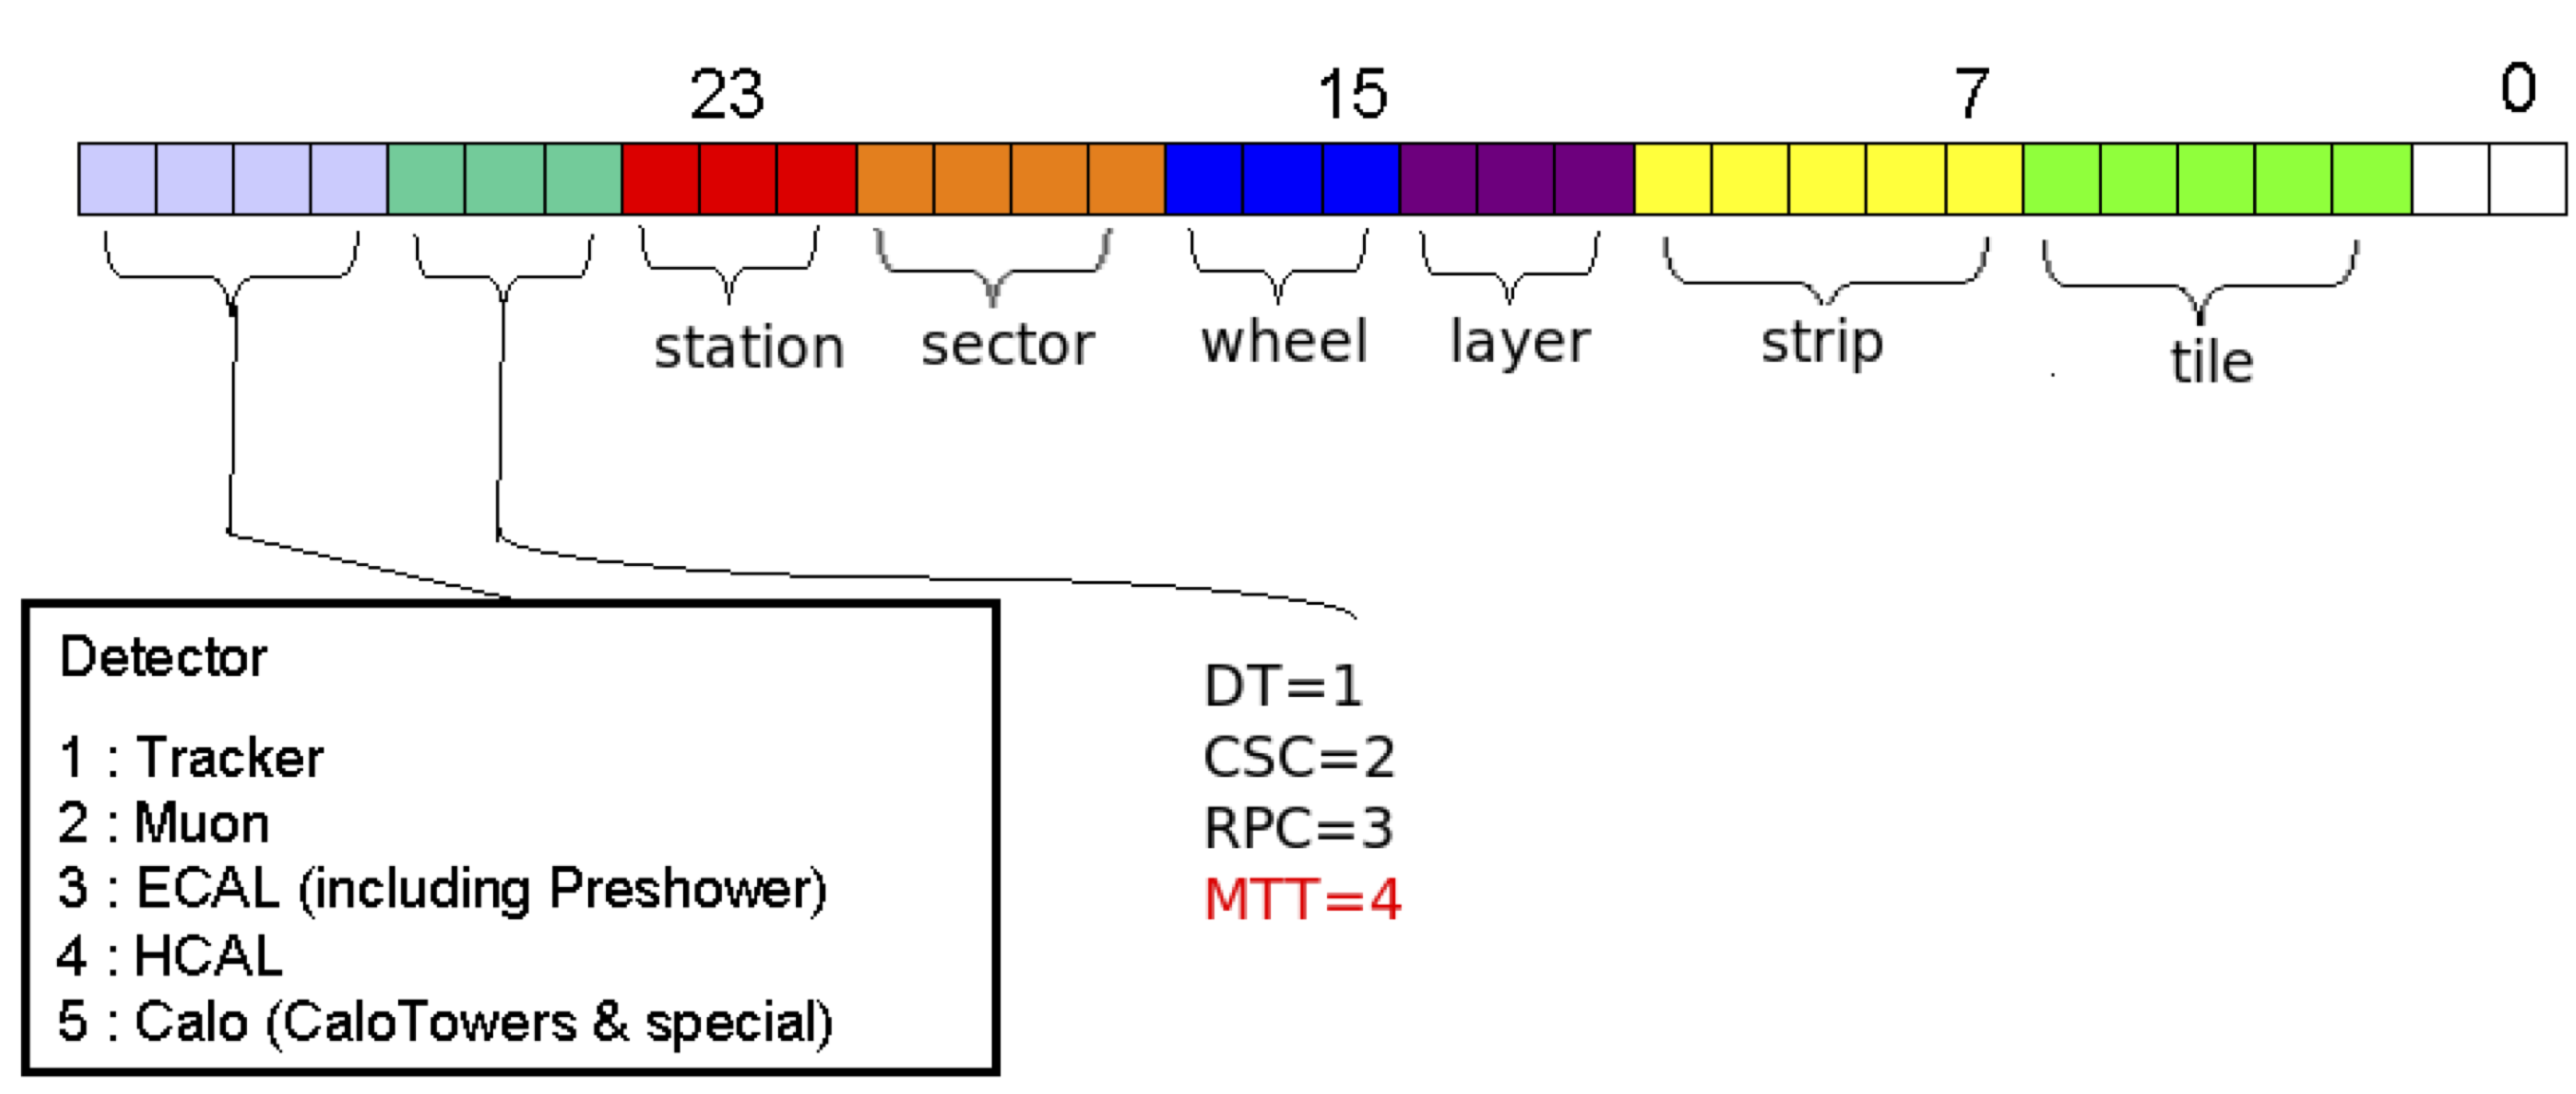
\includegraphics[width=0.70\textwidth]{Figures/erdogan/numbering.png}
				\caption{Unique numbering scheme of CMS detectors units.}
				\label{fig:numbering}
			\end{figure}
			The first four bits are reserved for the subdetector to which the considered detector unit belongs to.
			The following three bits are marking the subsystem within the subdetector, like DT, CSC, RPC or in our case MTT within the muon system.
			The remaining bits are used to desribe the location of the detector unit in a certain wheel, station etc.
			For MTT we used the three bits after the bits for the subsystem, for the station, four bits for the sector, three bits for the wheel, three bits for the layer, five bits for the strip and five bits
			for the tile.
			With this a MTT system consisting of seven layers each with 31 strips per $\varphi$-sector can be numbered consecutively in a unique way.
			This would allow tiles with only a few cm$^2$ surface area and since the planned MTT tiles are around 10$\times$10\,cm$^2$ this numbering is more than sufficient.
		\subsubsection{Setup and verification for the SimHit generation}
			After having the geometry of MTT within the CMSSW the next step is to create tools to simulate hits when particles go through a MTT tile.
			This task is handled by the \verb+MTTSensitiveDetector+ tool, which is based on the Geant4 counterpart SensitiveDetector.
			\verb+MTTSensitiveDetector+ collects the information like energy loss, time of flight or position step by step and stores it in a hit.
			Afterwards this tool has to be introduced to the general hit producer within CMSSW named the \verb+OscarProducer+.
			The \verb+OscarProducer+ is responsible for producing hits in several subdetectors at the beginning of an event.
			This is called the SIM step.
			(Furthermore the OscarProducer gives the subdetector algorithms constraints like energy thresholds etc.)
			To verify the correct behaviour of the MTT simhit generator, one can look at the position of the hits in the MTT tiles.
			For this purpose a muon gun placed in the point of origin of CMS was fired uniformly in all directions and the the x and y coordinates of the simulated hits in MTT were plotted (Fig.
			\ref{fig:hitpos_mtt}).
			\begin{figure}[htbp]
				\centering
				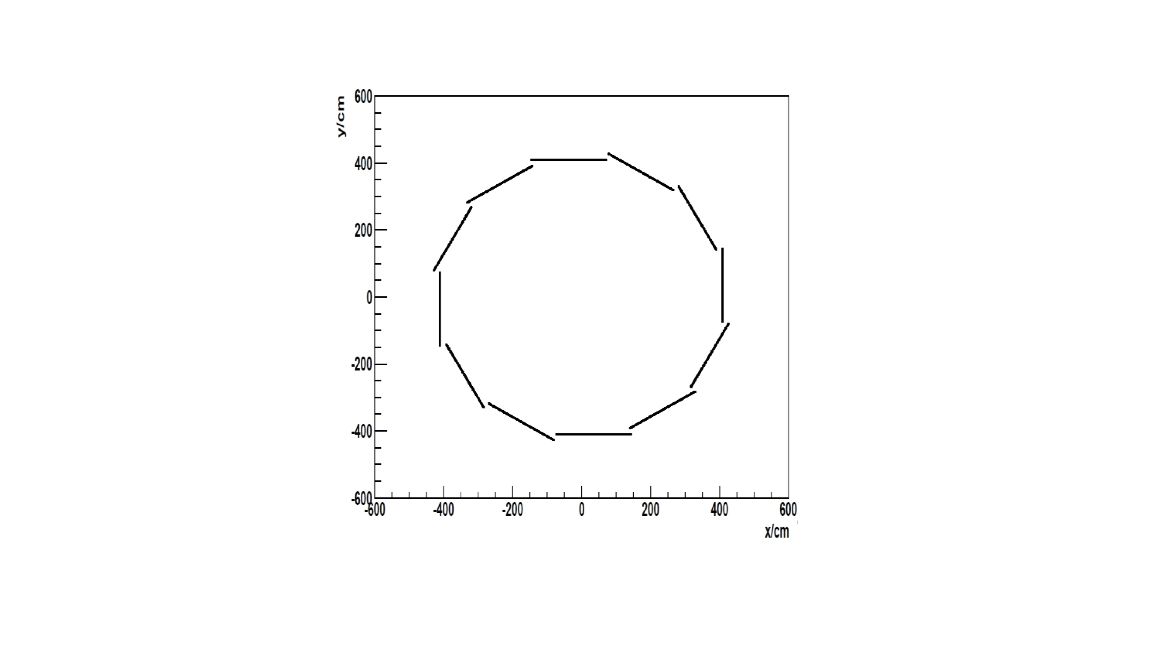
\includegraphics[width=0.70\textwidth]{Figures/erdogan/hitpos_mtt.png}
				\caption{Position of the hits simulated in the MTT in the x-y plane (from \cite{paul_thesis})}
				\label{fig:hitpos_mtt}
			\end{figure}
			The width of the 12 MTT panels in 12 $\varphi$ sectors can be seen at a distance of approximately four meters in x and y direction.
		\subsubsection{DIGI generation}
			The simulation of the hits with Geant4 based tools does not consider the detector response on the electronics site.
			This information has to be added to the simulation.
			This is called the DIGI step.
			Since the MTT tiles are under development and the front end electronics are not finalized yet, only a dummy digitizer could be written for MTT.
			In this dummy for each SimHit a DIGI is applied without any constraint on its parameters like energy or inefficiencies on the electronics site e.g. photon detection efficiency of the SiPMs etc.
			Nevertheless this digitizer is very important for the future analyzes since the MixingModule of CMSSW requires a digitizer to mix pile up information to the signal.
			Only with this it is possible to analyze the HL-LHC conditions with high pile up and with the extended CMS geometry by MTT.
%\subsection{First SimHit studies and their results}
	%All in this section shown first results are described in detail in (PAULREF).
	%As explained in the introduction chapter the main tasks for MTT would be the assignment of standalone muon tracks from the muon system to the tracks from track trigger (REF).
	%Therefore we have investigated the detection efficiency of L1Tracks in the MTT system.
	%However since the MTT system has only one layer with only 1 cm thickness, we don't expect very high efficiencies like the CMS muon system with its 4 stations and 4\,m lever arm can provide.
	%It is rather a feasibility analysis to see first hints of geometrical inefficiencies of the MTT.
	%In figure (REF) the matching efficiency as a function of transverse momentum $p_t$ of muons is depicted.
	%For this analysis a muon gun were used as described in the previous section.